\chapter{Symmetric instability in a cross-equatorial deep western boundary current}
\label{chap:4}
\begin{quote}
    \textit{So, does the staircase stay
    exactly as is, then?} --- Kevin McCloud, Grand Designs
\end{quote}

We have just seen how symmetric instability can be excited in a surface-intensified western boundary current as it crosses the equator, and you may wonder whether the findings of the preceding chapter apply to deep western boundary currents also. In this chapter, we will see that to some extent they do, and that symmetric instability may indeed be excited in cross-equatorial deep western boundary currents. We will explore how symmetric instability leads to the generation of density staircases in idealised models, potentially providing an easily observable fingerprint by which symmetric instability might be inferred observationally. We then go on to look at a simplified model of staircase formation and contrast what is going on in the Deep Western Boundary Current with what is going on in the surface North Brazil Current.

Ins section~\ref{sec:DWBCIntro} we will introduce the Deep Western Boundary Current in the Tropical Atlantic. In section~\ref{sec:methods} we describe our idealised numerical model of the Deep Western Boundary Current crossing the equator. In section~\ref{sec:randd} we demonstrate the formation of density staircases and the excitement of symmetric instability in the model, and propose that the staircases are generated as a result of the excitement of symmetric instability. Simple scaling arguments are used to explain the differences between the instabilities seen in deep western boundary currents and surface-intensified currents. Finally, in section~\ref{sec:conc} we summarise our findings and explain the potential implications of our results.

This chapter is based on a manuscript submitted to Geophysical Research Letters and has been accepted subject to revisions~\citep{Goldsworth2022}. I took the lead in the experimental design, implementation and authoring of the work.

\section{The Deep Western Boundary Current in the Tropical Atlantic}
\label{sec:DWBCIntro}
The Deep Western Boundary Current is the other major western boundary current system of the Tropical Atlantic. Unlike the North Brazil Current it is not driven by wind forcing and gyre circulations, rather, it is the main pathway of North Atlantic Deep Waters across the equator and into the Southern Ocean. Around $\flatfrac{2}{3}$rds of the AMOC's deep inter-hemispheric transport occurs in this current, with the remainder crossing the equator via interior pathways~\citep{Bower2019, Arhan1998}. The current has a peak velocity of around 20 cm\,s$^{-1}$, sits at a depth of approximately 1,200 m to 3,600 m and is around 100 km wide \citep{Rhein1995}. At 5$^\circ$S it transports $25.5\pm8.3$ Sv of water southwards \citep{Schott2005}. In the previous chapter, we saw how symmetric instability can be excited in surface intensified cross-equatorial western boundary currents; however, the susceptibility of deep western boundary currents to symmetric instability remains an open question. In the chapter, we will not only show that deep western boundary currents are susceptible to symmetric instability, but that this instability can result in the formation of density staircases.

Density staircases are step-like features which can be seen in plots of seawater density against depth, and they are ubiquitous in the global ocean \citep{Stern1960, Schmitt1987, Melling1984, Tait1968, Johannessen1974, Lambert1977}. The staircases consist of alternating well-mixed regions with low stratification and thin interfaces with high stratification. The high stratification interfaces act as ``mixing barriers'' which inhibit the vertical transport of water properties such as heat and salt, whereas mixing is enhanced in the low stratification regions. Density staircases can affect both diapycnal mixing and water mass transformation rates \citep{Schmitt2005}, which are known to be important in closing the AMOC's overturning budget \citep{DeLavergne2022}. Many staircases are thought to form as a result of double-diffusive convection \citep{Merryfield2000}, but other staircase generation mechanisms have been identified, such as inhomogeneous mixing~\citep{Balmforth1998}.



\section{Model configuration}
\label{sec:methods}

\begin{figure}[p]
    \centering
    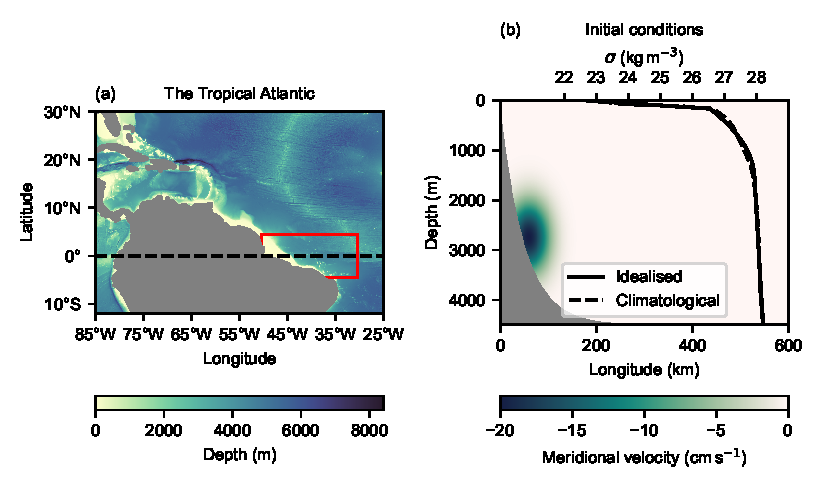
\includegraphics[width=\textwidth]{../figures/Figure1.pdf}
    \caption{(a) Bathymetric map of the western tropical Atlantic. Climatological profiles of neutral density were aggregated from the area enclosed by the red rectangle. Bathymetry data is from the \citet{GEBCO2020} dataset. (b) Meridional velocity (colours) and density (solid line) profiles used as initial and boundary conditions for the model. The velocity profile is based on observations by~\citet{Schott2005}, and the density profile on the climatological mean from~\citet{WOA2018} (dashed line).}
    \label{fig:fig1}
\end{figure}
Simulations of an idealised deep western boundary current crossing the equator are performed using the MITgcm~\citep{Marshall1997}. The domain size is 600 km in the zonal direction, 3,600~km in the meridional and 4,500~m in the vertical. The horizontal grid spacing is 1~km and the vertical grid spacing is 10~m. As with the models of the North Brazil Current, the horizontal resolution is chosen to ensure the model adequately resolves the small-scale vorticity dynamics we are studying and the vertical resolution is chosen to be smaller than the expected size of the overturning cells that symmetric instability generates\footnotemark. The time step is 144~s and the model is integrated for a total of 239~days. The longer integration time is chosen as the slower speeds of the Deep Western Boundary Current mean the model takes longer to spin up. The model domain is sited on a $\beta$-plane, with the equator placed 2,000~km north of the southern boundary. The meridional gradient in the Coriolis parameter is set to $2.3 \times 10^{-11}$ s$^{-1}\,$m$^{-1}$, and the meridional component of the Coriolis parameter is set to $1.5 \times 10^{-4}$ s$^{-1}$.
\footnotetext{A higher horizontal resolution is used here than in the North Brazil Current simulations, as at the time of the integrations being performed I was helping to test the ARCHER2 HPC facility before it came online. I had been instructed to try and push the system in terms of both the number of cores being used and the amount of data being produced. Ramping up the resolution was a simple (if not particularly creative) way of doing this.}

At the surface, a rigid lid boundary condition is employed. The lateral boundary conditions are set to be free-slip and the bottom boundary condition to no-slip. The model has sloping bathymetry as shown in figure~\ref{fig:fig1}b, which also shows the meridional velocity and density profiles used to initialise the model. The zonal velocity is initially set to zero. The density profile is based on a neutral density climatology aggregated from the area enclosed by the red rectangle in figure~\ref{fig:fig1}a. The model is forced by prescribing the meridional velocity, zonal velocity, and density, at the northern and southern domain boundaries. The same fields used to initialise the model are used as boundary conditions. A sponge region is placed at both the northern and southern edges of the domain. The northern sponge is 100 km thick and the southern sponge is 300~km thick. The inverse relaxation timescale varies from $1\times 10^{-5}$~s$^{-1}$ (corresponding to a timescale of around 1.2~days) at the external boundary of the sponge region to 0 at the model-sponge interface. The inverse relaxation timescale has a hyperbolic tangent shape, with a characteristic length scale of 5~km in the northern sponge and 10~km in the southern sponge.

As in chapter~\ref{chap:3}, a linear equation of state is used, with a reference density of 1022.73 kg\,m$^{-3}$ and thermal expansion coefficient of $2 \times 10^{-4}$ K$^{-1}$. The linear equation of state avoids the complexities added by non-linear effects such as thermobaricity and cabbelling~\citep[e.g.][]{Groeskamp2016}. The thermal diffusion coefficient is set to $1 \times 10^{-5}$ m$^{2}$\,s$^{-1}$. A second-order-moment Prather advection scheme with a flux limiter is employed. Salinity is set to be constant and has no impact on the dynamics. Momentum dissipation is provided by a vertical Laplacian viscosity of $4 \times 10^{-4}$ m$^{2}$\,s$^{-1}$ and an adaptive biharmonic Smagorinsky viscosity which acts on horizontal momentum gradients. Potential vorticity is calculated using the C-grid algorithm of~\citet{Morel2019}.

\section{Symmetric instability and staircase formation}
\label{sec:randd}
Figure~\ref{fig:staircase}b shows $\partial_z b$ in the model after 239 days of integration 250 km south of the equator. Immediately apparent are the thin, sharp regions of high stratification (so-called ``mixing barriers'') separating larger regions of well-mixed waters with low and uniform stratification. Moving to 500 km south, we see in figure~\ref{fig:staircase}c that some weaker barriers have dissipated, however, the stronger barriers remain. Figure~\ref{fig:staircase}a shows the squared buoyancy frequency at the equator. At the outer edge of the current's core, we see some weak mixing barriers.

\begin{figure}[t]
    \centering
    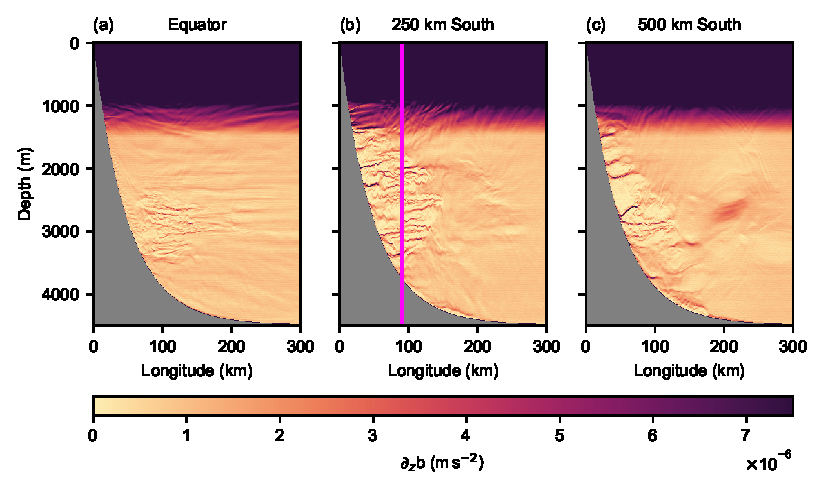
\includegraphics{../figures/Figure2.pdf}
    \caption{Squared buoyancy frequency after 239 days of model integration plotted at (a) the equator,  (b) 250 km south of the equator and (c) 500 km south of the equator. The magenta line indicates the location of the vorticity and density profiles shown in figure~\ref{fig:StaircaseMechanism}.}
    \label{fig:staircase}
\end{figure}

Figure~\ref{fig:StaircaseMechanism}a shows the average of the meridional component of relative vorticity between 234 and 239  days of model integration in a region 250 km south of the equator. This can be thought of as a crude proxy for a zonal overturning stream function --- it measures the local rotation around the meridional axis, i.e. the amount of zonal overturning. As the flow is not invariant in the meridional direction, the ``true'' zonal overturning stream function is ill-defined, so here we will consider the meridional vorticity instead. Examining the meridional vorticity, note that there are a series of counter-rotating stacked overturning cells between around 1,750 m and 3,500 m below the surface. The black contours overlain show $\partial_z b = 2 \times 10^{-6}$~s$^{-2}$ and help identify the locations of the mixing barriers in figure~\ref{fig:staircase}b. We can see that the structure of the buoyancy frequency squared and the meridional vorticity are remarkably similar, with the horizontal edges of the overturning cells (vorticity zeros) approximately coinciding with the locations of the mixing barriers. This can also be seen in figure~\ref{fig:StaircaseMechanism}b. The black line shows neutral density plotted as a function of depth at 250 km south and 90 km west (the location of the magenta lines and points shown in the other figures). The orange line shows the meridional component of relative vorticity at the same point. Both quantities have been averaged over the period spanning 234 to 239 days. The treads of the steps in neutral density correspond to mixing barriers and the risers to well-mixed regions. When comparing neutral density and the meridional vorticity we again see that the mixing barriers tend to coincide with vorticity zeros, whereas the mixing barriers coincide with vorticity extrema. This suggests that the inhomogeneous mixing driven by the overturning cells is what is causing the formation of the staircases.

\begin{figure}[p]
    \centering
    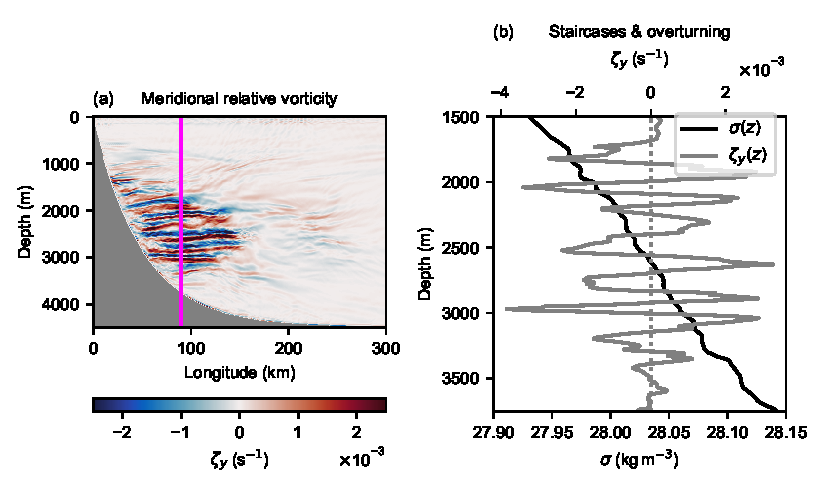
\includegraphics{../figures/Figure3.pdf}
    \caption{(a) The time mean meridional component of relative vorticity between 234 and 239 days of model integration, plotted as a function of longitude and depth, at 250 km south. Overlain is the contour defined by $\partial_z b = 2 \times 10^{-6}$~s$^{-2}$, indicating locations of mixing barriers. (b) Density (black line) and the time mean meridional component of relative vorticity (orange line) plotted as a function of depth at 90 km west and 250 km south (shown on other figures as a magenta line or point). Panels (c) to (e) show snapshots of the stratification over time from the toy model. The contours on panel (c) show the overturning stream function used to drive staircase formation.}
    \label{fig:StaircaseMechanism}
\end{figure}

\subsection{A very simple model of staircase formation}
The differential mixing which produces the mixing barriers is analogous to the process which produces zonal jets on a $\beta$-plane \citep{Manfroi1999}. \citet{Manfroi1999} study a sheared zonal flow on a $\beta$-plane and find that mixing in the presence of a meridional gradient in planetary vorticity leads to the preferential formation of zonal jets. The separation of the jets is set by the strength of the mixing. Here, instead of a meridional gradient in planetary vorticity, there is a vertical gradient in buoyancy and instead of mixing in the horizontal plane we have overturning in the vertical plane. We can reproduce the formation of mixing barriers with a toy model, in which we consider how buoyancy changes over time as a result of vertical diffusion and advection by overturning cells. If we express the overturning motion as a stream-function $\psi$ where $u = - \partial_z \psi$ and $w = \partial_x \psi$ and use a constant harmonic diffusivity, $\kappa$ we can express the evolution of $b$ as
% TODO: Do we need to reparamaterise this now we're using a variable diffusivity?
\begin{equation}
    \frac{\partial b}{\partial t} = \frac{\partial \psi}{\partial z} \frac{\partial b}{\partial x} - \frac{\partial \psi}{\partial x} \frac{\partial b}{\partial z} + \kappa \frac{\partial^2 b}{\partial z^2} \, .
\end{equation}
This is the advection-diffusion equation of a passive tracer in a two-dimensional flow. We choose $\psi = e^{- x^2 / 2\delta_x^2} \sin(m z)$, to represent stacked overturning cells which are localised to a region of width $\delta_x$ in the horizontal. We also set $b(t=0) = N^2 z$, and then solve the equation numerically using the 3rd order Adam's Bashforth scheme on a domain stretching from $-50$~km to $50$~km in the horizontal and spanning $600$~m in the vertical. We set $\delta_x = 25$~km, $m = 2 \pi / 200$ m$^{-1}$, $\kappa = 1 \times 10^{-5}$~m$^2$\,s$^{-1}$ and $N^2 = 1 \times 10^{-6}$~s$^{-2}$. The grid spacing is set to 1 km in the horizontal and 2.5 m in the vertical, and the time step is 240 seconds. In regions where the stratification is unstable, $\kappa$ is increased to $5 \times 10^{-3}$~m$^2$\,s$^{-1}$.

The stratification in this toy model is shown at three different times in figures~\ref{fig:StaircaseMechanism}c to \ref{fig:StaircaseMechanism}e. Alternating high and low stratification regions develop with time. Initially, this is a result of differential mixing; however, at later times the mixing barriers become sharper and start to form filaments due to the extra mixing occurring in regions with unstable stratification.

% TODO: Make the profile point smaller
\begin{figure}[p]
    \centering
    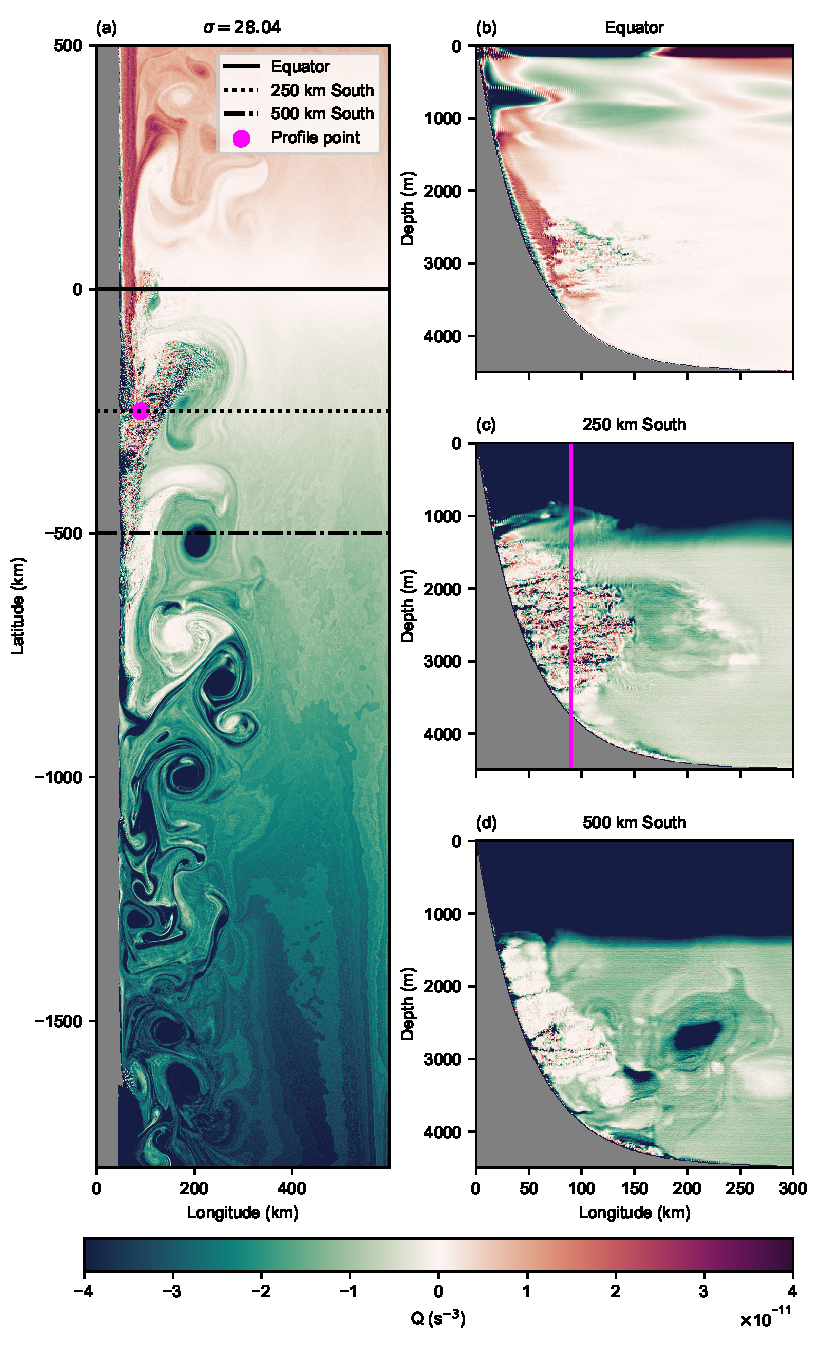
\includegraphics{../figures/Figure4.pdf}
    \caption{Potential vorticity after 239 days of model integration plotted on (a) the $\gamma^n = 28.04$ surface, (b) at the equator, (c) at 250 km south of the equator, and (d) at 500 km south of the equator. Black lines show the latitudes at which sections have been plotted. The magenta line and point indicate the location of the vorticity and density profiles shown in figure~\ref{fig:StaircaseMechanism}.}
    \label{fig:PV}
\end{figure}

\subsection{But what is generating the overturning?}
In chapter~\ref{chap:3}, we saw that western boundary currents can become unstable when crossing the equator as they advect anomalous potential vorticity from one hemisphere into the other. In figure~\ref{fig:PV}a, which shows the potential vorticity on the $\gamma^n$ = 28.04 surface, we can see the advection of positive potential vorticity from the Northern Hemisphere into the Southern Hemisphere, so we may expect to see symmetric instability excited south of the equator. The excitement of the instability is apparent in a region from around 25 km to 600 km south of the equator. Figures~\ref{fig:PV}b to \ref{fig:PV}d show the potential vorticity as a function of depth and longitude at, the equator, 250 km south and 500 km south respectively, after 239 days of model integration. At the equator, we see the advection of waters with anomalous potential vorticity into the Southern Hemisphere. At 250 km south we can see the excitement of symmetric instability, and by 500 km south we can see large pools of neutral potential vorticity suggesting the waters here have experienced symmetric instability, with the excitement of symmetric instability still underway at around 3,000 m. In figure~\ref{fig:PV}b we also see symmetric instability-like patterns in a region of negative potential vorticity. This suggests these waters with negative potential vorticity were undergoing symmetric instability in the Northern Hemisphere before being advected south of the equator. This also explains the presence of the weak staircases at the equator seen in figure~\ref{fig:staircase}a. A similar mechanism was proposed by \citet{DOrgeville2004} in their investigation of deep zonal jets along the equator.

\subsection{Estimating at which latitudes symmetric instability occurs}
\label{sec:relation2nbc}
In the Deep Western Boundary Current, we see the excitement of symmetric instability close to the equator followed by the formation of eddies, unlike in the North Brazil Current where we see the spinning up of large anti-cyclonic eddies followed by the excitement of symmetric instability further away from the equator. This is due to the reduced growth rate of barotropic instability in the deep western boundary current~\citep{Edwards1998II}, meaning that symmetric instability dominates over short time scales. In the North Brazil Current the anti-cyclonic eddies act to reduce the growth rate of symmetric instability further, allowing anomalous potential vorticity to persist whilst the eddies grow~\citep{Buckingham2021}. 

We can be more quantitative about the latitude at which the instability is forming. There is an e-folding timescale, $\tau_e$, associated with symmetric instability which can be converted into an advective meridional length scale, $y$ with the equation $y = V \tau_e$, where V is a typical meridional velocity. From linear stability theory, we know that for a parallel shear flow, like a deep western boundary current the timescale of symmetric instability is given by
\begin{equation}
    \tau_e \sim \Bigg(\beta y \bigg(f + \frac{V}{L_x}\bigg) \Bigg)^{-1/2}
\end{equation}
\citep{Hoskins1974}, and that for the case of an eddy, such as a North Brazil Current ring, the symmetric instability timescale is
\begin{equation}
    \tau_e \sim \Bigg(\beta y \bigg(f + \frac{2 V}{R}\bigg) \Bigg)^{-1/2}
\end{equation}
\citep{Buckingham2021}. We can then convert these expressions to a meridional length scale, giving
\begin{equation}
    y \sim \sqrt[3]{\frac{V L_x}{\beta}} \, ,
    \label{eq:dwbc_y}
\end{equation}
for parallel shear flows, and for an eddy
\begin{equation}
    y \sim \sqrt[3]{\frac{2 V R}{\beta}} \, .
    \label{eq:nbc_y}
\end{equation}
In the case of the eddying flow, we have assumed the meridional velocity is of a similar order of magnitude to the azimuthal velocity. In both expressions, we have assumed $y$ to be small and only considered terms of the lowest order in $y$. We can now evaluate the expressions for the latitude of the onset of symmetric instability. For the Deep Western Boundary Current we choose $V \sim 0.2$ m\,s$^{-1}$, $L_x \sim 30$ km and $\beta \sim 2.3 \times 10^{-11}$~m$^{-1}$\,s$^{-1}$, giving $y \sim 60$ km. For the North Brazil Current rings we choose $V \sim 1$~m\,s$^{-1}$, $R \sim 100$~km and the same value for $\beta$, giving $y \sim 200$ km. These predictions of the latitude of instability are of the same order of magnitude as those we see in the numerical models. In the case of North Brazil Current rings, we see instability at around 400 km north, and in the Deep Western Boundary Current, we see instability from around 25 km south of the equator.

\section{Summary}
\label{sec:conc}
Density staircases are step-like features which become apparent when density is plotted as a function of depth and are common throughout the Earth's oceans. In an idealised model of a deep western boundary current crossing the equator, we see density staircases form. The staircases are generated by overturning cells which are in turn generated by the excitement of symmetric instability as the current crosses the equator. Symmetric instability in cross-equatorial flows is excited due to the advection of anomalous potential vorticity from one hemisphere to another. The stacked overturning cells that generate the staircases are, however, a feature of symmetric instability regardless of what is forcing it, suggesting we may see staircase formation in other symmetrically unstable flows, including when anomalous potential vorticity is induced by frictional torques or diabatic processes. Differences in the latitude of instability between surface intensified western boundary currents and deep western boundary currents can be adequately explained using simple scaling arguments relating the growth rate of symmetric instability to the currents' advective timescales.

It is thought that diapycnal mixing may play an important role in closing the overturning budget of the Atlantic Meridional Overturning Circulation's deep limb. Figures~\ref{fig:staircase} and~\ref{fig:PV} clearly show that vigorous mixing is taking place; however, accurately calculating the amount of mixing that is occurring is tricky. This is due to the importance of secondary Kelvin Helmholtz instabilities in transforming water masses. In order to resolve these processes, we would need a model with around 40 times the resolution used here \citep{Bachman2014}, which is computationally infeasible --- such a model would require at least $10^4$ times more computational resources to run. Simplified two-dimensional models may help in accurately quantifying the induced diapycnal mixing, however.

Density staircases are well documented in the Tropical Atlantic and are often said to form as a result of salt fingering and double diffusive convection (e.g.~\citet{Schmitt1987, Schmitt2005}). In light of this work, we suggest new insights into mixing in the region could be gained by revisiting existing observations and re-examining the origins of observed staircases.
